% Section name and highlighted ToC
\renewcommand{\sectiontitle}{Introduction}
\section{\sectiontitle}
\customToC{currentsection,hideothersubsections}{}

% Section name and highlighted ToC
\renewcommand{\subsectiontitle}{What is machine learning?}
\subsection{\subsectiontitle}

% Bishop definition of machine learning
\begin{frame}{\subsectiontitle}
    As it is said in the introduction of chapter one in  \cite{BishopPatternRecognition}
 \textbf{machine learning} \textit{is the field of pattern 
recognition that is concerned with the automatic
 discovery of regularities in data and the use of
these regularities to take actions such as 
classifying the data into different categories}.
\end{frame}

% --- Math formulation 
% 1. Naive perspective 
\renewcommand{\subsectiontitle}{Math formulation}
\customToC{currentsection,hideothersubsections}{}
\subsection{\subsectiontitle}
\begin{frame}{\subsectiontitle}
    Let be
    \begin{itemize}
        \item an input vector $X \in \mathbb{R}^d$, 
        \item and out-put function $Y \in \mathbb{R}$.
    \end{itemize}
    
    \textbf{ 
      We seek a function $f(X)$ for predicting $Y$ given values of the input $X$.
      }
\end{frame}
% 2. Emphasized joint distribution
\begin{frame}{\textbf{My new} math formulation \footnote{ From \cite{HastieStatisticalLearing}}}
    Let be
    \begin{itemize}
        \item an input vector: $X \in \mathbb{R}^d$, 
        \item an out-put function: $Y \in \mathbb{R}$,
        \item  \textbf{with joint distribution $Pr(X,Y)$}.
    \end{itemize}
    
      We seek a function $f(X)$ for predicting $Y$ given values of the input $X$.

      \pause 
      \begin{theorem}{The idealistic function}
        
      \end{theorem}  
      Exist a function $f: \mathbb{R}^d \longrightarrow \mathbb{R}$ that maps perfectly 
      every element of $(x,y) \in X \times Y$ ie 
      \begin{equation}
        \forall (x,y) \in X \times Y 
        \quad
        f(x) = y 
        \Longleftrightarrow
        P(y |X=x) = 1.
      \end{equation}

      \textbf{This is stricter than say they are $Pr(x,y)$ connected}.
    \end{frame}
\begin{frame}{Definition of linear regression}
  Basic definition of a lineal model: 
    \begin{equation}
      y(x,w) = x \cdot w^T
    \end{equation}
    where $x \in \{1\}\times\R^{d}$ and $w \in \R^{d+1}$. 
\end{frame}

\begin{frame}{Problems of global polinomial function}
  \textbf{Runge's phenomenon}\footnote{Sources: 
  General overview of approximation theory \cite{ACourseInApproximationTheory} 
  and Wikipedia \cite{Splines} and \cite{RungePhenomenon}}
  \begin{figure}
    \centering
    \begin{subfigure}[b]{0.4\textwidth}
        \centering
        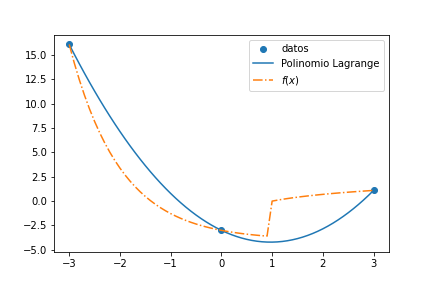
\includegraphics[width=\textwidth]{02_Lineal_models/lagrange-3-datos.png}
        \caption[]%
        {{\small Lagrange polynomial of three nodes}}    
        \label{fig:mean and std of net14}
    \end{subfigure}
    \hfill
    \begin{subfigure}[b]{0.4\textwidth}   
        \centering 
        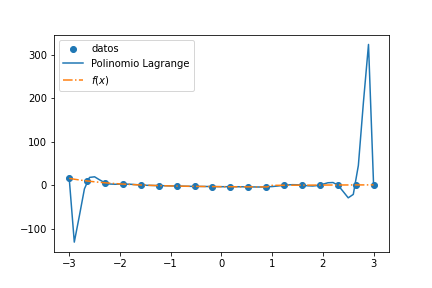
\includegraphics[width=\textwidth]{02_Lineal_models/lagrange-18-datos.png}
        \caption[]%
        {{\small Lagrange polynomial of 18 nodes}}    
        \label{fig:}
    \end{subfigure}
    \caption[ The error converges to infinity]
    {\small The error converges to infinity} 
    \label{fig:01errorToInfinty}
  \end{figure}
\end{frame}

\begin{frame}{Explantation}
  Runge's phenomenon is the consequence of two properties of this problem: 
  \begin{enumerate}
    \item   The magnitude of the n-th order derivatives of this particular function grows quickly when n increases.
    \item   The equidistance between points leads to a Lebesgue constant that increases quickly when n increases. \footnote{Source: \cite{LebesgueConstant}} (Lagrange Base Polynomial)
  \end{enumerate}

  Solutions: 
  \begin{enumerate}
    \item Controlling derivatives: \textbf{Splines} (Solve 1).
    \item Reducing the domain where a variable could effect \textbf{basic functions}(Solve 2).
  \end{enumerate}

  More aproachs??? \textcolor{red}{I need to read \cite{ACourseInApproximationTheory}}
\end{frame}

\begin{frame}
  \frametitle{Generalization of lineal models}

  It can be generalized as: 
    \begin{equation}
      y(x,w) = \phi(x) \cdot w^T
    \end{equation}
    where $\phi_j(x)$ are known as \textbf{basic functions}. 

    (Notation: $\phi_0(x) = w_0$ is usually known as \textbf{bias}). 

\end{frame}

\begin{frame}
  \frametitle{Some values of basic functions}
  \begin{center}
    \begin{tabular}{ |c| c| c |}
      \hline
     Gaussian & Logistic sigmoid & Wavelets\footnote{Read more at 
     \cite{Wavelet} and \cite{ACourseInApproximationTheory}} \\ 
     \hline
     $exp \left(-\frac{(x-\mu)^2}{2 \sigma^2}\right)$
     & % Sigmoid formula
     $\frac{1}{1 + \exp(\frac{x-\mu}{\sigma})}$  
    & $c \sum (-1)^i \sin(2^i \pi x)$ \\  
     % images 
     % 1. Gaussian
     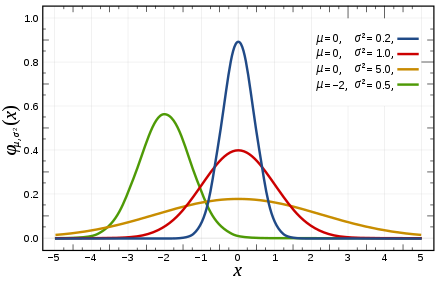
\includegraphics[width=.3\textwidth]{02_Lineal_models/gaussian_function.png}
      & % 2. Sigmoid function 
      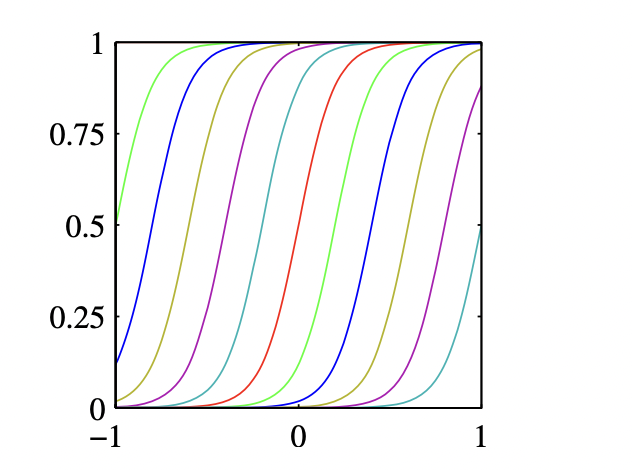
\includegraphics[width=.3\textwidth]{02_Lineal_models/sigmoid_function.png}
      & 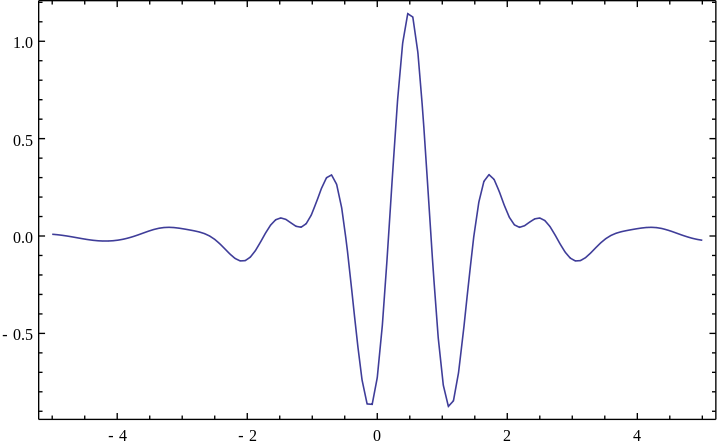
\includegraphics[width=.3\textwidth]{02_Lineal_models/MeyerMathematica.png} \\
     \hline  
    \end{tabular}
    \end{center}
\end{frame}

\begin{frame}
  \frametitle{Least Squeres}
  How good is our approximation?

  We also showed that this error function could 
  be motivated as the maximum likelihood 
  solution under an assumed Gaussian noise model.
  

\end{frame}